\begin{frame}
    \frametitle{Performance Measures - Number of individuals}
    \centering

    \begin{tikzpicture}
        \node[state] (my_state) {\((u_i,v_i)\)};
        \node[right=of my_state] (pi_state) {\( \pi_{(u_i,v_i)} \)}; 
        \draw[every loop] (my_state) edge (pi_state);
    \end{tikzpicture}
    \pause

    \begin{equation*}
        L = \sum_{i=1}^{|\pi|} \pi_{i} (u_i + v_i) 
    \end{equation*}
    \begin{equation*}
        L_1 = \sum_{i=1}^{|\pi|} \pi_{i} v_i 
    \end{equation*}
    \begin{equation*}
        L_2 = \sum_{i=1}^{|\pi|} \pi_{i} u_i 
    \end{equation*}

\end{frame}


\begin{frame}
    \frametitle{Performance Measures - Waiting time}
    \centering

    \begin{equation*}
        W = \frac{\lambda_1 P_{L'_1}}{\lambda_2 P_{L'_2} + \lambda_1 P_{L'_1}} W^{(1)} 
        + \frac{\lambda_2 P_{L'_2}}{\lambda_2 P_{L'_2} + \lambda_1 P_{L'_1}} W^{(2)}
    \end{equation*}

    \begin{equation*}
        W^{(1)} = \frac{\sum_{\substack{(u,v) \, \in S_A^{(1)} \\ v \geq C}} 
        \frac{1}{C \mu} \times (v-C+1) \times \pi(u,v)}{\sum_{(u,v) \, 
        \in S_A^{(1)}} \pi(u,v)}
    \end{equation*}
        
    \begin{equation*}
        W^{(2)} = \frac{\sum_{\substack{(u,v) \, \in S_A^{(2)} \\ min(v,T) \geq C}} 
        \frac{1}{C \mu} \times (\min(v+1,T)-C) \times \pi(u,v)}{\sum_{(u,v) \, 
        \in S_A^{(2)}} \pi(u,v)}
    \end{equation*} 

\end{frame}


\begin{frame}
    \frametitle{Performance Measures - Waiting time}

    \scriptsize
    \begin{equation*}
        W^{(1)} = \frac{\sum_{(u,v) \in S_A^{(1)}} w^{(1)}(u,v) 
        \pi_{(u,v)}}{\sum_{(u,v) \in S_A^{(1)}} \pi_{(u,v)}},
        \quad
        W^{(2)} = \frac{\sum_{(u,v) \in S_A^{(2)}} w^{(2)}(u,v) \pi_{(u,v)}}
        {\sum_{(u,v) \in S_A^{(2)}} \pi_{(u,v)}}
    \end{equation*}
    \vspace{1cm}
    \tiny
    \pause
    \begin{equation*}
        S_A^{(1)} = \{(u, v) \in S \; | \; v < N \}, 
        \quad
        S_A^{(2)}=
        \begin{cases}
            \{(u, v) \in S \; | \; u < M \} & \textbf{if } T \leq N\\
            \{(u, v) \in S \; | \; v < N \} & \textbf{otherwise}
        \end{cases}
    \end{equation*}
    
    \pause
    \begin{equation*}
        S_W = \{(u, v) \in S \; | \; v > C \}    
    \end{equation*}

    \pause
    \begin{equation*}
        c^{(1)}(u,v) = 
        \begin{cases}
            0, & \textbf{if } u > 0 \textbf{ and } v = T \\
            \frac{1}{\text{min}(v,C)\mu}, & \textbf{otherwise}
        \end{cases}, 
        \quad
        c^{(2)}(u,v) = 
        \begin{cases}
            0, & \textbf{if } u > 0 \\
            \frac{1}{\text{min}(v,C)\mu}, & \textbf{otherwise}
        \end{cases}
    \end{equation*}
    \pause
    \begin{equation*}
        w^{(i)}(u,v) = 
        \begin{cases} 
            0, & \textbf{if } (u,v) \notin S_w \\
            c^{(i)}(u,v) + w^{(i)}(u-1, v), & \textbf{if } u > 0 \textbf{ and } v = T \\
            c^{(i)}(u,v) + w^{(i)}(u, v-1), & \textbf{otherwise}
        \end{cases}
    \end{equation*}

\end{frame}


\begin{frame}
    \frametitle{Performance Measures - Blocking time}
    \centering
    \begin{equation*}
        B = \frac{\sum_{(u,v) \in S_A^{(2)}} \pi_{(u,v)} \; 
        b(u,v)}{\sum_{(u,v) \in S_A^{(2)}} \pi_{(u,v)}}
    \end{equation*}

\end{frame}


\begin{frame}
    \frametitle{Performance Measures - Blocking time}

    \scriptsize
    \begin{equation*}
        B = \frac{\sum_{(u,v) \in S_A^{(2)}} \pi_{(u,v)} \; 
        b(u,v)}{\sum_{(u,v) \in S_A^{(2)}} \pi_{(u,v)}}
    \end{equation*}

    \tiny
    \pause
    \begin{equation*}
        b(u,v) = 
        \begin{cases} 
            0, & \textbf{if } (u,v) \notin S_b \\
            c(u,v) + b(u - 1, v), & \textbf{if } v = N = T\\
            c(u,v) + b(u, v-1), & \textbf{if } v = N \neq T \\
            c(u,v) + p_s(u,v) b(u-1, v) + p_a(u,v) b(u, v+1), & \textbf{if } u > 0 
            \textbf{ and } \\ 
            & \quad v = T \\
            c(u,v) + p_s(u,v) b(u, v-1) + p_a(u,v) b(u, v+1), & \textbf{otherwise} \\
        \end{cases}
    \end{equation*}
    
    \pause
    \begin{equation*}
        S_b = \{(u,v) \in S \; | \; u > 0\}
    \end{equation*}
        
    \pause
    \begin{equation*}
        c(u,v) = 
        \begin{cases}
            \frac{1}{\min(v,C) \mu}, & \text{if } v = N\\
            \frac{1}{\lambda_1 + \min(v,C) \mu}, & \text{otherwise}
        \end{cases}
    \end{equation*}
    
    \pause
    \begin{equation*}
        p_s(u,v) = \frac{\min(v,C)\mu}{\lambda_1 + \min(v,C)\mu}, \qquad
        p_a(u,v) = \frac{\lambda_1}{\lambda_1 + \min(v,C)\mu}
    \end{equation*}
    
\end{frame}


\begin{frame}
    \frametitle{Performance Measures - Proportion within time}
    \centering
    
    \small
    \begin{equation*}
        P(X < t) = \frac{\lambda_1 P_{L'_1}}{\lambda_2 P_{L'_2}+\lambda_1 P_{L'_1}} 
        P(X^{(1)} < t) + \frac{\lambda_2 P_{L'_2}}{\lambda_2 P_{L'_2} + 
        \lambda_1 P_{L'_1}}P(X^{(2)} < t) 
    \end{equation*}

    \begin{equation*}
        P(X^{(1)} < t) = \frac{\sum_{(u,v) \in S_A^{(1)}} P(X_{(u,v)}^{(1)} < t) 
        \pi_{u,v} }{\sum_{(u,v) \in S_A^{(1)}} \pi_{u,v}}
    \end{equation*}
    
    
    \begin{equation*}
        P(X^{(2)} < t) = \frac{\sum_{(u,v) \in S_A^{(2)}} P(X_{(u,v)}^{(2)} < t) 
        \pi_{u,v} }{\sum_{(u,v) \in S_A^{(2)}} \pi_{u,v}}
    \end{equation*}
    
\end{frame}


\begin{frame}
    \frametitle{Performance Measures - Proportion within time}

    \scriptsize
    \begin{equation*}
        P(X^{(i)} < t) = \frac{\sum_{(u,v) \in S_A^{(i)}} P(X_{u,v}^{(i)} < t) 
        \pi_{u,v} }{\sum_{(u,v) \in S_A^{(i)}} \pi_{u,v}}, \quad \textbf{for } i = \{1, 2\}
    \end{equation*}

    \only<1>{
        \vspace{6.15cm}
    }
    
    \pause
    \only<2>{
        \tiny
        \vspace{0.9cm}
        \begin{equation*}
            P(X_{(u,v)}^{(1)} < t) = 
            \begin{cases}
                1 - \sum_{i=0}^{v-1} \frac{1}{i!} e^{-\mu t} (\mu t)^i, 
                & \textbf{if } C = 1 \textbf{ and } v>1 \\
                1 - (\mu C)^{v-C} \mu  
                    \sum_{k=1}^{\mid \vec{r} \mid} \sum_{l=1}^{r_k}
                    \frac{\Psi_{k,l}(-\lambda_k)t^{r_k - l} 
                    e^{-\lambda_k t}}{(r_k - l)! (l - 1)!},
                & \textbf{if } C > 1 \textbf{ and } v > C \\
                    \qquad \textbf{where } \vec{r}=(v - C, 1) \textbf{ and } 
                    \vec{\lambda}=(C \mu, \mu) &  \\
                1 - e^{-\mu t},  & \textbf{if } v \leq C
            \end{cases}
        \end{equation*}
        \vspace{0.9cm}
        \begin{equation*}
            P(X_{(u,v)}^{(2)} < t) = 
            \begin{cases}
                1 - \sum_{i=0}^{\min(v,T)-1} \frac{1}{i!} e^{-\mu t} (\mu t)^i,  
                & \textbf{if } C = 1 \textbf{ and } v, T > 1 \\
                1 - \mu (\mu C) ^ {\min(v,T) - C} \times 
                    \sum_{k=1}^{\mid \vec{r} \mid} \sum_{l=1}^{r_k} 
                    \frac{\Psi_{k,l}(-\lambda_k)t^{r_k - l} 
                    e^{-\lambda_k t}}{(r_k - l)! (l - 1)!}, 
                & \textbf{if } C > 1 \textbf{ and } v, T  > C \\
                    \qquad \textbf{where } \vec{r}=(\min(v, T) - C, 1) 
                    \textbf{ and } \vec{\lambda}=(C \mu, \mu) \\
                1 - e^{-\mu t}, & \textbf{if } v \leq C 
                    \textbf{ or } T \leq C \\
            \end{cases}
        \end{equation*}
        \vspace{0.85cm}
    }
    
    \only<3>{
        \vspace{1cm}
        \begin{equation*}
            X_{(u,v)}^{(1)} \sim 
            \begin{cases}
                \textbf{Erlang}(v, \mu), & \textbf{if } C = 1 \textbf{ and } v>1 \\
                \textbf{Hypo} \left(
                    \left[v - C, 1\right], \left[C \mu, \mu \right]
                \right), & \textbf{if } C > 1 \textbf{ and } v>C \\
                \textbf{Erlang}(1, \mu), & \textbf{if } v \leq C
            \end{cases}
        \end{equation*}
        \vspace{1cm}
        \begin{equation*}
            X_{(u,v)}^{(2)} \sim 
            \begin{cases}
                \textbf{Erlang}(\min(v, T), \mu), & \textbf{if } C = 1
                    \textbf{ and } v, T > 1 \\
                \textbf{Hypo}\left(
                    \left[ \min(v, T) - C, 1 \right], \left[ C \mu, \mu \right]
                \right), & \textbf{if } C > 1 \textbf{ and } v, T  > C \\
                \textbf{Erlang}(1, \mu), & \textbf{if } v \leq C \textbf{ or } T \leq C
            \end{cases}
        \end{equation*}
        \vspace{1.1cm}
    }
    

\end{frame}


\begin{frame}
    \frametitle{Comparisons}

    \begin{multicols}{3}
        % Overall
        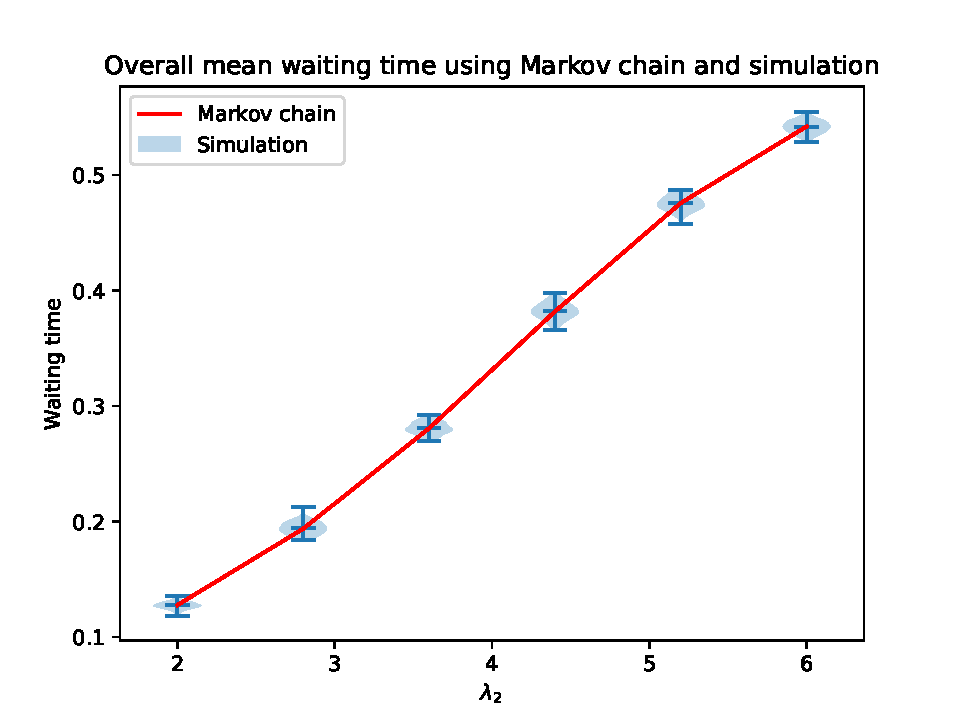
\includegraphics[scale=0.2]{Bin/performance_measures_comparison/waiting_overall_comparison.pdf}
        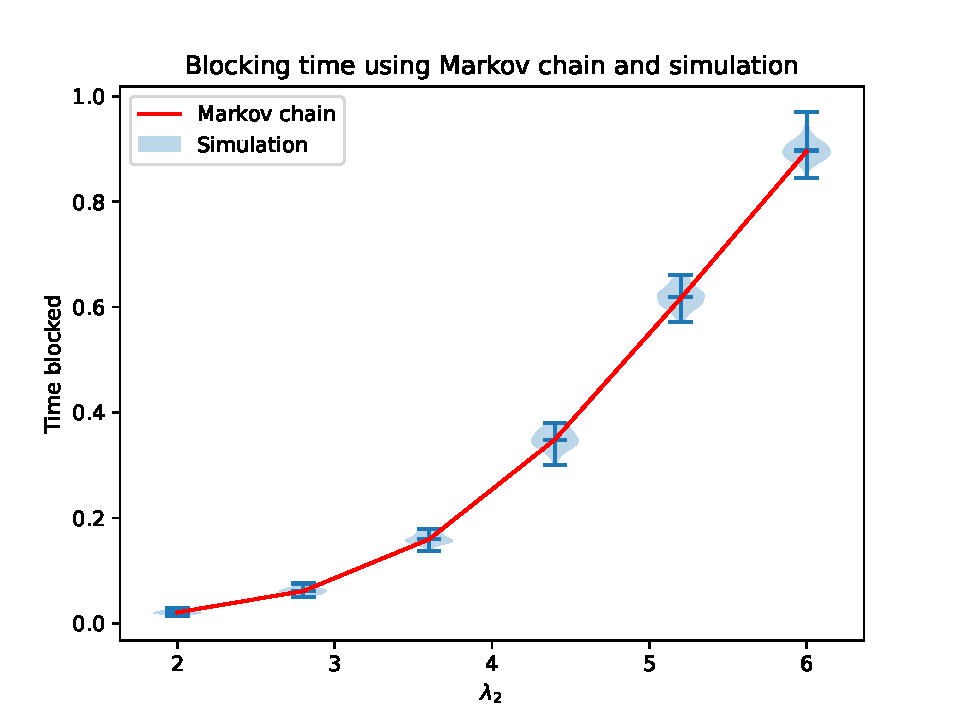
\includegraphics[scale=0.2]{Bin/performance_measures_comparison/blocking_comparison.pdf}
        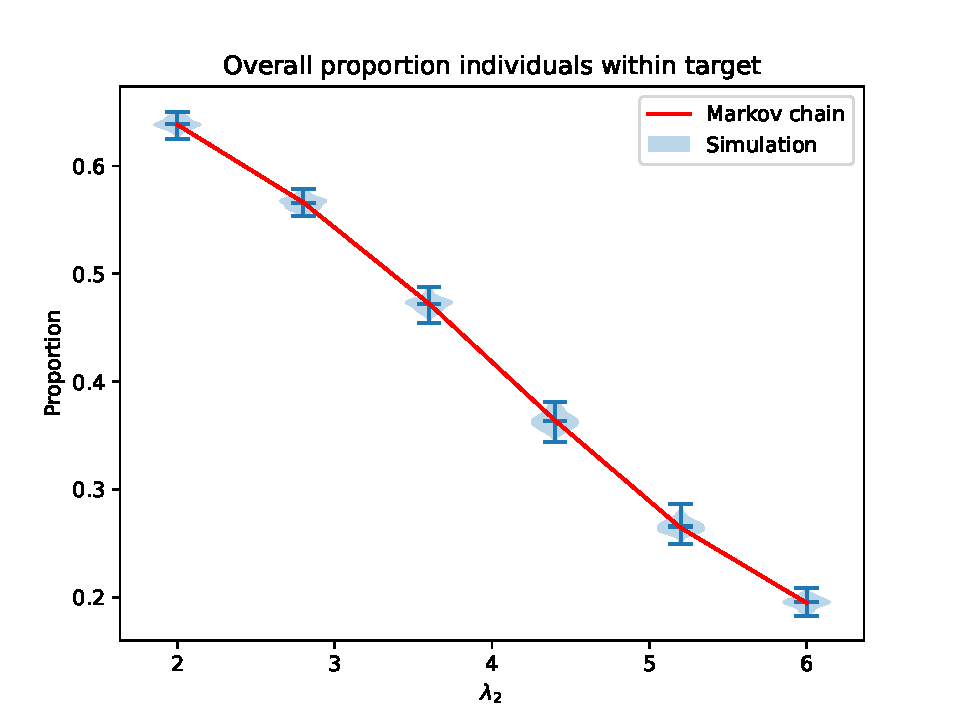
\includegraphics[scale=0.2]{Bin/performance_measures_comparison/proportion_overall_comparison.pdf}
        
        \columnbreak
        % Type 1
        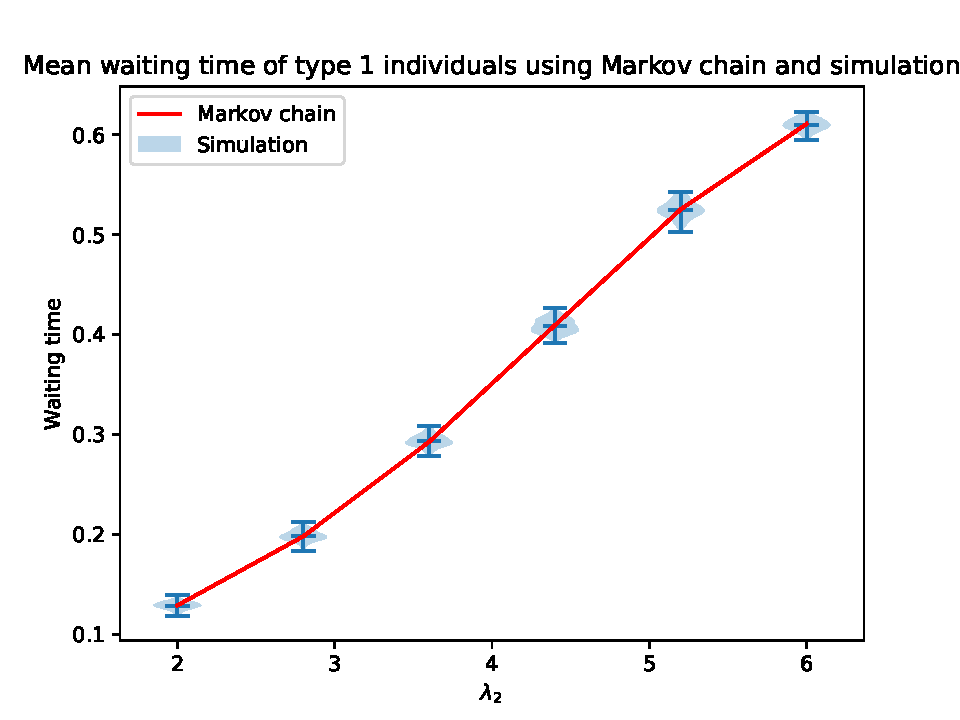
\includegraphics[scale=0.2]{Bin/performance_measures_comparison/waiting_1_comparison.pdf}

        \vspace{2.5cm}
        
        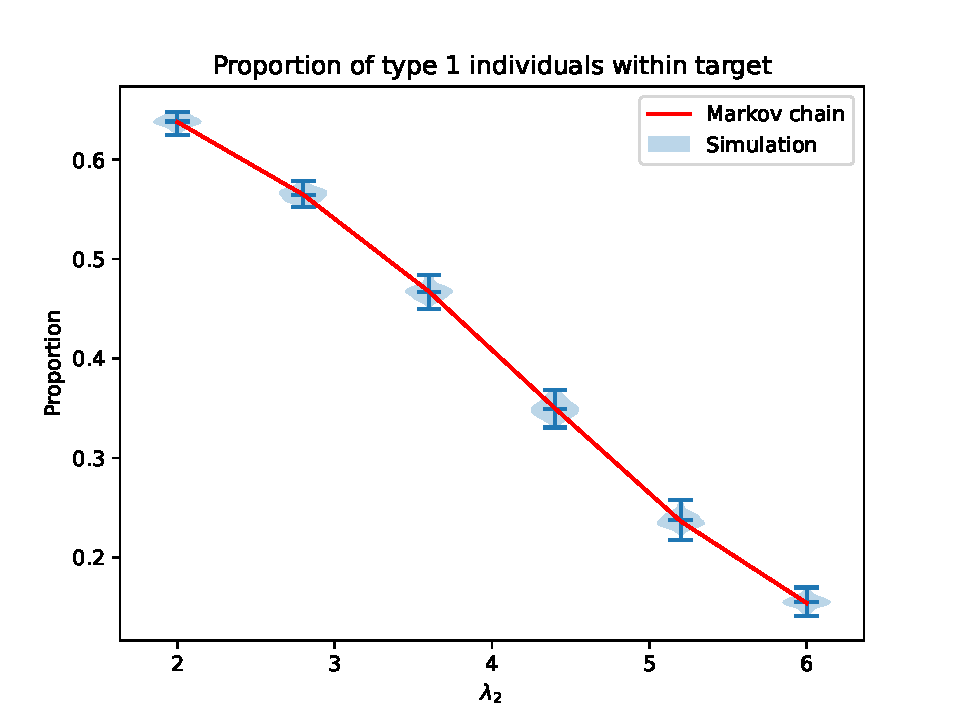
\includegraphics[scale=0.2]{Bin/performance_measures_comparison/proportion_1_comparison.pdf}
        
        \columnbreak
        % Type 2
        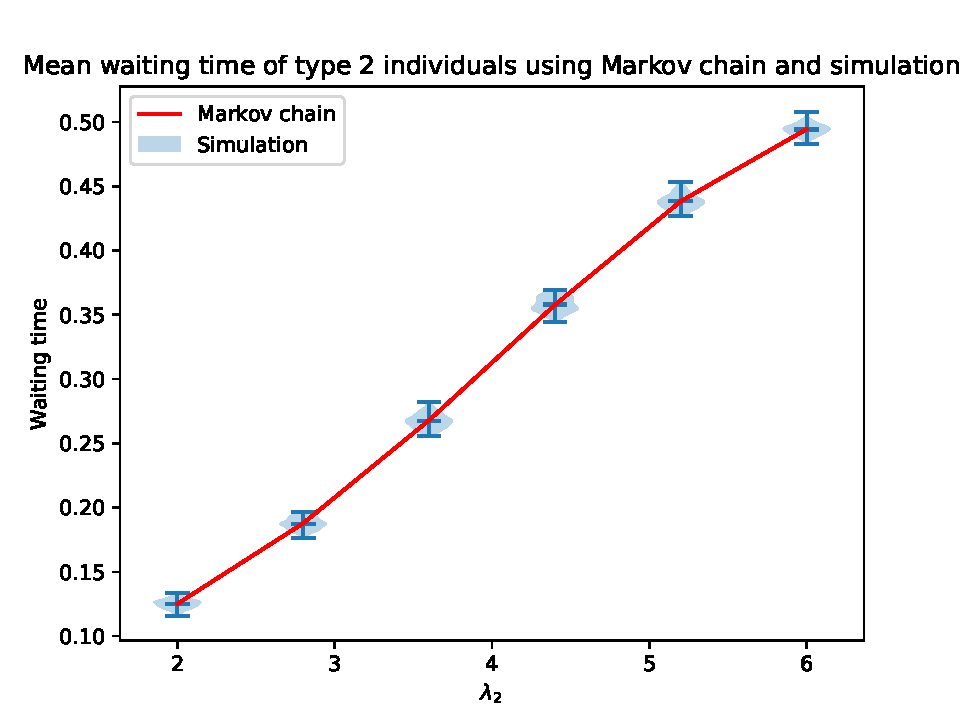
\includegraphics[scale=0.2]{Bin/performance_measures_comparison/waiting_2_comparison.pdf}
        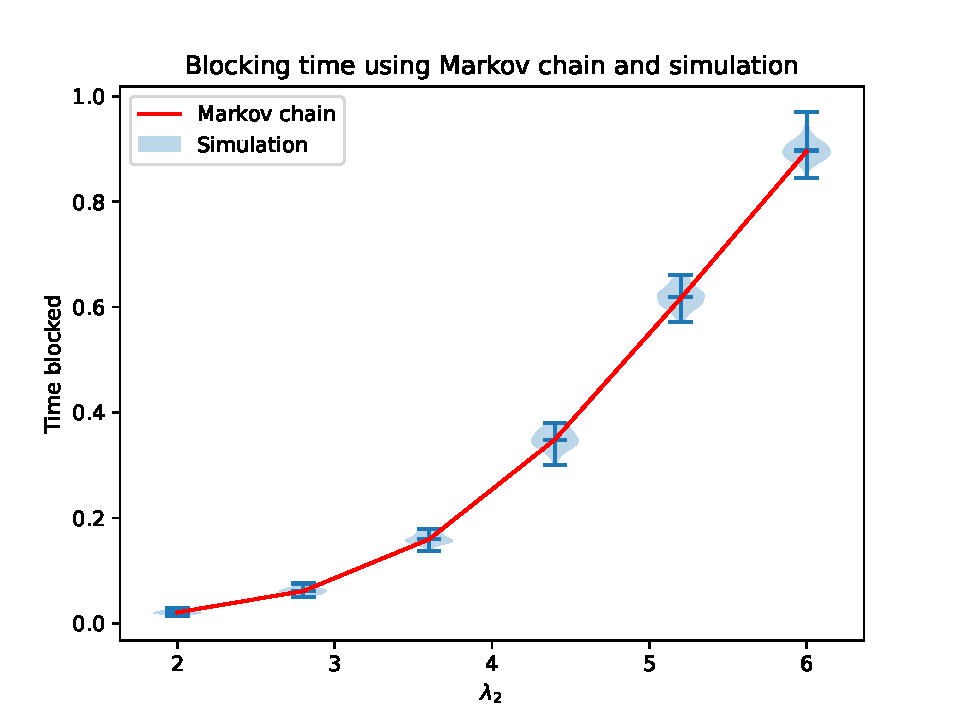
\includegraphics[scale=0.2]{Bin/performance_measures_comparison/blocking_comparison.pdf}
        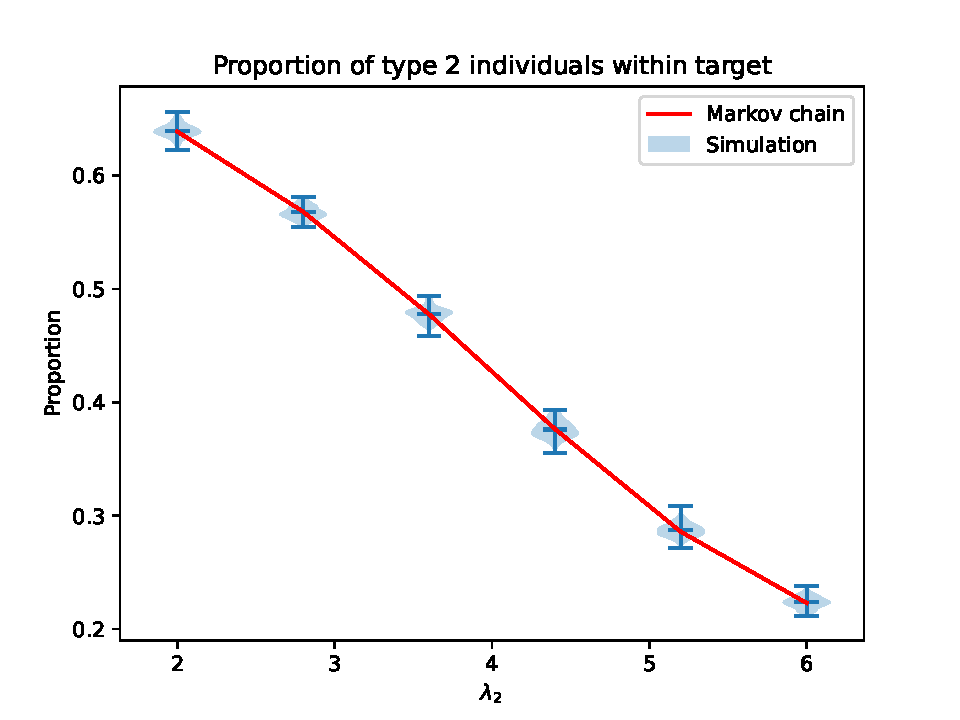
\includegraphics[scale=0.2]{Bin/performance_measures_comparison/proportion_2_comparison.pdf}
    \end{multicols}


\end{frame}